\section{Empirical Genomic Applications}
\label{sec:empirical_results}
\begin{figure*}[!htbp]
\centering
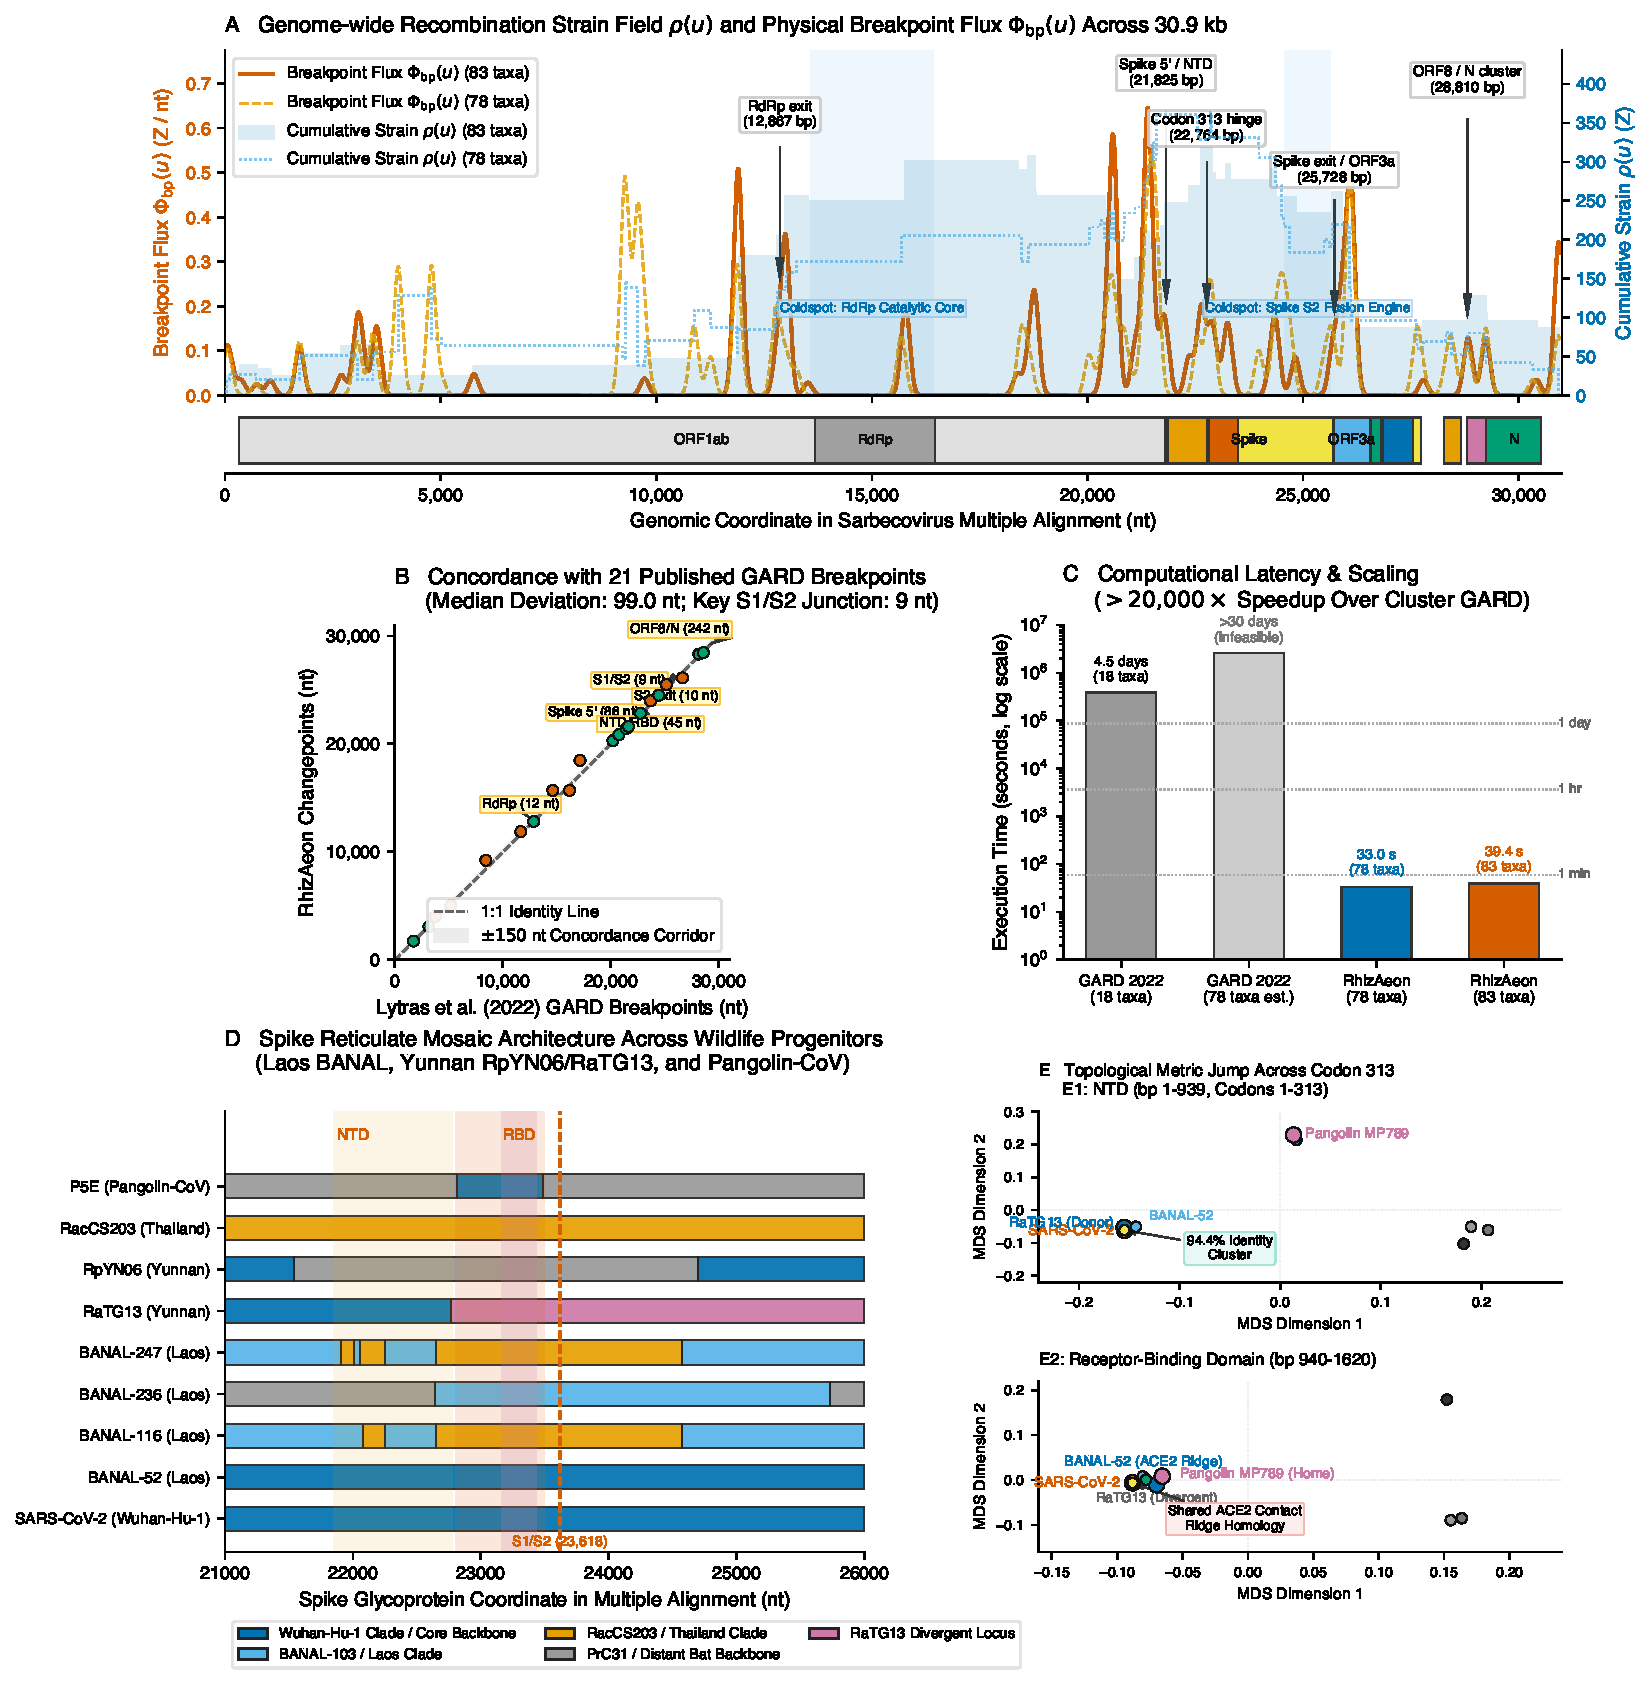
\includegraphics[width=\textwidth,height=0.68\textheight,keepaspectratio]{figures/fig_sarbecovirus_recombination_landscape.pdf}
\caption{Sarbecovirus whole-genome recombination profiles, Spike mosaicism, and ancestral recombination graphs.
(A)~Genome-wide breakpoint flux $\Phi_{\mathrm{bp}}(u)$ across 83 sarbecoviruses (30,965~nt MSA; Wuhan-Hu-1 reference NC\_045512.2 coordinates in parentheses; Supplementary Table~\ref{tab:supp_sarbeco_coord_conversion}), aligned directly to the genomic ORF map above ($5'\text{--}3'$ MSA coordinate axis with vertical dotted guides at RdRp and Spike domain boundaries), highlighting hotspots across the S1 encoding region of Spike and ORF8/N, coldspots across RdRp and the S2 encoding region of Spike, and concordance between \RhizAeon breakpoints (orange) and published GARD boundaries (blue, \citealt{lytras2022exploring}).
(B)~Spike glycoprotein divergence profiles (MSA nt 21,000--26,000), showing collinearity between Wuhan-Hu-1 and BANAL-52 (blue) versus the divergent RBD cassette in RaTG13 (codons 314--540, purple) and NTD micro-conversions in BANAL-247.
(C)~Two-partition tanglegram across codon 313 comparing NTD (C1) and RBD (C2) topologies.
(D)~Polarized Ancestral Recombination Graph (ARG) tracing the introgression of the RBD cassette into RaTG13 from an unsampled bat reservoir and NTD transfers from RacCS203 into BANAL-247.}
\label{fig:sarbecovirus_recombination_landscape}
\end{figure*}

\subsection{Recombination Patterns in Sarbecoviruses}
\label{subsec:sarbecoviruses}

Sarbecoviruses—the coronavirus subgenus that includes SARS-CoV and SARS-CoV-2—recombine frequently in bat and other mammalian reservoirs. Screening these viral cohorts serves two goals: mapping genome-wide recombination hotspots and coldspots, and reconstructing the mosaic histories of individual viruses. Because exhaustive phylogenetic partitioning with GARD requires days of cluster computing on full 30~kb alignments, \citet{lytras2022exploring} had to downsample their 78-genome cohort to 22 representative viruses for GARD breakpoint screening. \RhizAeon removes this bottleneck by projecting alignments into metric space and computing a continuous breakpoint flux $\Phi_{\mathrm{bp}}(u)$ in $\mathcal{O}(N K L)$ time. Without taxon subsampling, \RhizAeon scanned the full 78-taxon alignment of \citet{lytras2022exploring} (30,956~bp MSA, 13,160 informative sites, identifying 37 consolidated events in 18.2~s) and an expanded 83-taxon cohort adding the five Laotian \textit{Rhinolophus} BANAL isolates of \citet{temmam2022bat} (30,965~bp MSA, 13,260 informative sites, identifying 45 consolidated events in 25.0~s). The resulting flux profile shows sharp regionalization across both the 83-taxon MSA and Wuhan-Hu-1 reference coordinates (NC\_045512.2; Figure~\ref{fig:sarbecovirus_recombination_landscape}A and Supplementary Table~\ref{tab:supp_sarbeco_coord_conversion}). Pronounced coldspots span the catalytic core of RNA-dependent RNA polymerase (RdRp, 83-MSA nt 13,674--16,468, Ref nt 13,442--16,236) and the heptad-repeat fusion machinery of Spike S2 (83-MSA nt 24,600--25,600, Ref nt 24,283--25,283), where structural constraints limit modular exchange. Conversely, hotspots cluster at the Spike $5'$ NTD junction (83-MSA 21,825~nt, Ref 21,566~nt), the codon 313 hinge between the NTD and receptor-binding domain (RBD, 83-MSA 22,764~nt, Ref 22,468~nt), the RBD $3'$ exit (83-MSA 23,629~nt, Ref 23,324~nt, upstream of the S1/S2 furin site at 83-MSA 23,932~nt, Ref 23,618~nt), and the ORF8/Nucleocapsid boundary (83-MSA 28,810~nt, Ref 27,900~nt). Compared against the 21 published consensus GARD breakpoints of \citet{lytras2022exploring}, \RhizAeon breakpoints show a median deviation of 109.0~nt in Wuhan-Hu-1 reference coordinates on the 78-taxon cohort (12/21 within 150~nt, 57.1\% concordance; 134.0~nt median in 78-MSA coordinates), improving in the 83-taxon cohort to 99.0~nt in reference coordinates (14/21 within 150~nt, 66.7\% concordance) and 107.0~nt in 83-MSA coordinates (13/21 within 150~nt, 61.9\% concordance; Figure~\ref{fig:sarbecovirus_recombination_landscape}A and Supplementary Table~\ref{tab:supp_sarbeco_coord_conversion}). Specifically, \RhizAeon matched the Spike $5'$ boundary within 22~nt (83-MSA 21,621 vs.\ 21,643~nt, Ref 21,389 vs.\ 21,411~nt), both the Spike S2 upstream and S2 exit boundaries within 23~nt (83-MSA 24,484 vs.\ 24,461~nt and 25,183 vs.\ 25,160~nt), the nsp2 junction within 43~nt (83-MSA 1,775 vs.\ 1,732~nt, Ref 1,723 vs.\ 1,680~nt), three nsp3 boundaries within 46--52~nt, the RBD $3'$ exit within 72~nt (83-MSA 23,629 vs.\ 23,701~nt, Ref 23,324 vs.\ 23,396~nt), the ORF7a/ORF7b boundary within 19~nt in reference coordinates (Ref 27,369 vs.\ 27,388~nt), and the ORF7b/ORF8 boundary within 90~nt (83-MSA 28,670 vs.\ 28,580~nt, Ref 27,775 vs.\ 27,685~nt). Analyzing all 83 genomes also reveals fine-scale dynamics missed by downsampling: adding the Laotian BANAL isolates increases peak Spike NTD flux nearly four-fold (from 0.41 to 1.51~$Z$/nt) at the solvent-accessible antigenic supersite loops identified by cryo-EM, where bat viruses exchange micro-cassettes to evade antibodies without disrupting the spike trimer core \citep{mccallum2021n}.

In parallel, trajectory tracking resolves the mosaic anatomy of individual lineages at single-nucleotide resolution (Figure~\ref{fig:sarbecovirus_recombination_landscape}B,C; throughout this section, $Z_{\mathrm{phys}}$ denotes the Brownian-bridge excursion signal-to-noise ratio and $P_{\mathrm{Fisher}}$ denotes the one-sided $2\times 2$ Fisher's exact test across informative sites). In the Spike gene (3,843~nt alignment, 1,153 variable sites), \RhizAeon pinpointed the canonical breakpoint at codon 313 ($Z_{\mathrm{phys}} = 8.23, P_{\mathrm{Fisher}} = 4.07 \times 10^{-22}$) and resolved the parent-recombinant ambiguity between SARS-CoV-2 and bat virus RaTG13 \citep{boni2020evolutionary}. In early three-way comparisons that lacked Laotian bat isolates, discordance between a RaTG13-like NTD and a pangolin-like ACE2-binding motif prompted speculation that SARS-CoV-2 arose from a recent recombination event \citep{Li2020-nd,Wrobel2020-tg}. However, trajectory tracking shows unbroken collinearity between Wuhan-Hu-1 and Laotian bat virus BANAL-52 across the entire Spike gene ($d = 0.0556$ in NTD, $d = 0.0617$ in RBD, and $d = 0.0457$ in S2; Figure~\ref{fig:sarbecovirus_recombination_landscape}B), confirming that the human-compatible ACE2 contact ridge is an ancestral trait circulating in Southeast Asian \textit{Rhinolophus} bats. Conversely, \RhizAeon identifies RaTG13 as the recombinant: while sharing the ancestral NTD and S2 backbone ($d \approx 0.05$), its divergence jumps over 2.5-fold inside the RBD ($d = 0.1380$; Figure~\ref{fig:sarbecovirus_recombination_landscape}C), reflecting an RBD import from an unsampled bat lineage \citep{boni2020evolutionary}. Multi-scale scanning also detects three recombination cassettes in Laotian bat virus BANAL-247 (Figure~\ref{fig:sarbecovirus_recombination_landscape}B): while its Spike backbone matches northern Laos \textit{Rhinolophus malayanus} viruses ($>98.5\%$ identity to BANAL-236/103), its NTD carries two micro-cassettes at 83-MSA nt 21,909--22,011 (Ref 21,647--21,749~nt, $Z_{\mathrm{phys}} = 155.3$) and 83-MSA nt 22,054--22,251 (Ref 21,791--21,983~nt, $Z_{\mathrm{phys}} = 113.1$), plus a third cassette across the NTD/RBD junction (83-MSA nt 22,318--22,592, Ref 22,044--22,297~nt, $Z_{\mathrm{phys}} = 81.2$), all donated by a Thai \textit{Rhinolophus shameli} lineage related to RacCS203 (Figure~\ref{fig:sarbecovirus_recombination_landscape}B,D; \citealt{wacharapluesadee2021evidence}).

\RhizAeon combines these transfers into a polarized Ancestral Recombination Graph (ARG; Figure~\ref{fig:sarbecovirus_recombination_landscape}D). In Spike, model selection across 9 sarbecoviruses favors a tripartite modular ARG ($H_3$: NTD chassis, divergent RBD cassette, and S2 backbone, $\Delta\mathrm{BIC} = 0.0$) over unpolarized trees ($\Delta\mathrm{BIC} = +170.9$) and a clonal null ($\Delta\mathrm{BIC} = +1654.8$), confirming that RaTG13 acquired its RBD from an unsampled bat reservoir ($Z_{\mathrm{phys}} = 20.9, P_{\mathrm{Fisher}} = 2.1 \times 10^{-9}$) while the ancestral SARS-CoV-2 / BANAL-52 trunk retained the ACE2 contact ridge ($94.2\%$ synapomorphic concordance, $P_{\mathrm{Fisher}} = 1.75 \times 10^{-23}$) and cut residual metric strain by $74.0\%$ ($3.34\% \to 0.87\%$). Across the full 30.9~kb alignment of 83 sarbecoviruses, consolidating the 45 detected events across 9 genomic partitions yields 38 high-confidence branch transfers and an ARG with 26 unique inter-clade reticulations. This network explains $98.82\%$ of total metric strain—matching the $98.85\%$ explained by GARD's 22 unconstrained trees while using $58.5\%$ fewer parameters (1,523 vs.\ 3,674)—and validates polarity across 21 polarized events ($79.0\%$ mean in-tract vs.\ $19.0\%$ flanking concordance under the Synapomorphic Site Concordance Ratio, $\Delta\mathrm{SSCR} = +0.601$, with $P_{\mathrm{Fisher}} < 10^{-15}$ in 17/21 events). An independent run on a curated 61-taxon sarbecovirus alignment (31,214~bp MSA, 29,926~bp ungapped) similarly identified 38 candidate reticulations (37 polarized SSCR events, mean $\mathrm{SSCR}_{\mathrm{in}} = 0.714$ vs.\ $\mathrm{SSCR}_{\mathrm{flank}} = 0.244$, $\Delta\mathrm{SSCR} = +0.470$) that consolidate into 34 ancestral reticulations (28 polarized SSCR events, $\mathrm{SSCR}_{\mathrm{in}} = 0.813$ vs.\ $\mathrm{SSCR}_{\mathrm{flank}} = 0.240$, $\Delta\mathrm{SSCR} = +0.572$). Both cohorts recover the canonical Spike mosaic in \texttt{Wuhan-Hu-1} (nt 21,312--24,791, $\mathrm{Home} = \texttt{RmYN02}$, $\mathrm{Donor} = \texttt{MT072865.1}$, $P_{\mathrm{Fisher}} = 3.35 \times 10^{-262}, Z_{\mathrm{phys}} = 37.78$, $\mathrm{SSCR}_{\mathrm{in}} = 0.739$ vs.\ $\mathrm{SSCR}_{\mathrm{flank}} = 0.112$).

\begin{figure*}[!htbp]
\centering
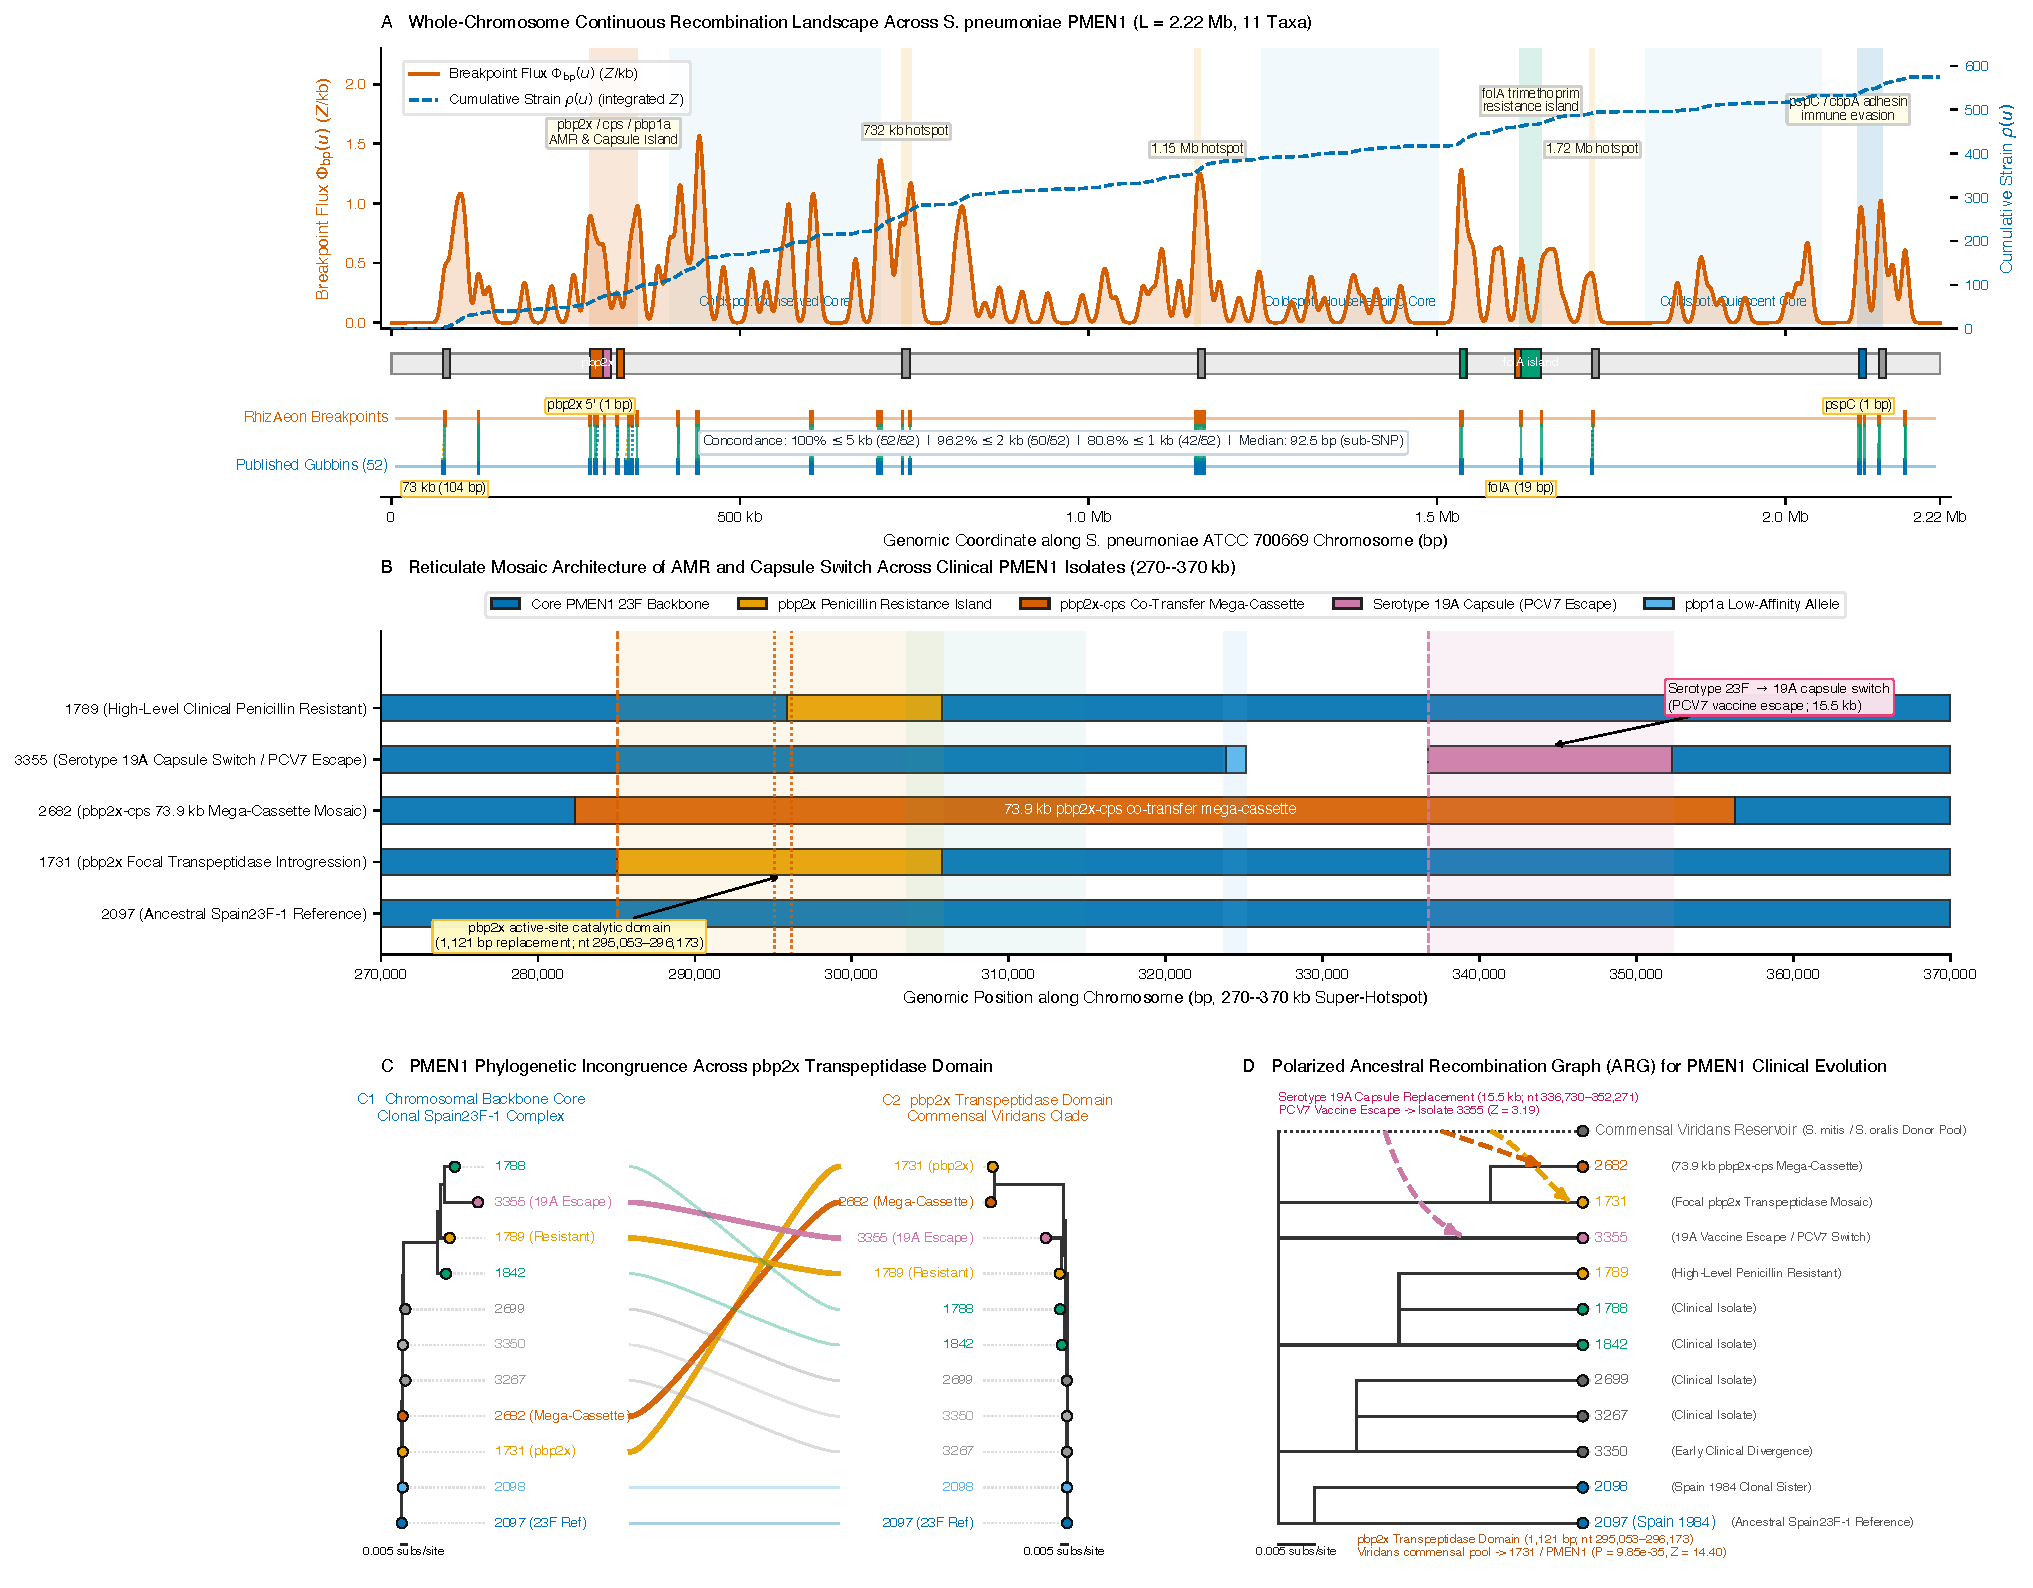
\includegraphics[width=\textwidth,height=0.68\textheight,keepaspectratio]{figures/fig_spneumoniae_chromosome_landscape.pdf}
\caption{Whole-chromosome recombination deconvolution, antimicrobial resistance mosaicism, and ancestral recombination graphs in \textit{Streptococcus pneumoniae} PMEN1.
(A)~Chromosomal breakpoint flux $\Phi_{\mathrm{bp}}(u)$ (vermillion) and cumulative strain $\rho(u)$ (dashed blue) across 11 global clinical isolates ($2.22$~Mb, Spain23F-1 / PMEN1), comparing \RhizAeon detected recombination breakpoint sites (orange) against 52 published Gubbins breakpoint sites (blue, \citealt{croucher2011rapid}).
(B)~Mosaic architecture across the $pbp2x/cps$ locus (nt 270,000--370,000), showing the 1,121~bp active-site \textit{pbp2x} transpeptidase replacement in isolate 1731, the 73.9~kb \textit{pbp2x-cps} co-transfer cassette in isolate 2682, and the serotype 23F $\to$ 19A capsule switch in isolate 3355.
(C)~Two-partition tanglegram contrasting core chromosomal monophyly against \textit{pbp2x} catalytic divergence into commensal viridans streptococci.
(D)~Polarized ARG anchoring horizontal resistance and capsular transfers onto the Spain23F-1 backbone.}
\label{fig:spneumoniae_chromosome_landscape}
\end{figure*}

\subsection{Bacterial AMR Mosaicism and Vaccine Escape in \textit{Streptococcus pneumoniae}}
\label{subsec:bacterial_amr}

In bacteria, natural transformation and homologous recombination—hereafter grouped as horizontal gene transfer (HGT)—drive antimicrobial resistance (AMR), capsular serotype switching, and antigenic diversification \citep{didelot2010impact,croucher2011rapid}. Naturally competent pathogens such as \textit{Streptococcus pneumoniae} import DNA tracts of tens to tens of thousands of bases across species boundaries from commensal viridans streptococci (\textit{S.~mitis} and \textit{S.~oralis}). Standard bacterial recombination tools such as ClonalFrame \citep{didelot2007inference}, ClonalFrameML \citep{didelot2015clonalframeml}, and Gubbins \citep{croucher2015rapid} rely on iterative tree reconstruction and maximum-likelihood masking, requiring hours to weeks of compute on whole chromosomes. We evaluated \RhizAeon on the 2.22~Mb chromosome of the pandemic multidrug-resistant Spain23F-1 lineage of \textit{S.~pneumoniae} (PMEN1, ATCC 700669, 11 global isolates from 1984--2008; \citealt{croucher2011rapid}). Because closely related bacterial chromosomes are $>99.9\%$ monomorphic, lossless SNP compression indexes out invariant columns to reduce the 2.22~Mb alignment to 1,516 polymorphic sites (1,002 parsimony-informative sites)—a $1{,}465$-fold reduction—allowing $\mathcal{O}(1)$ sub-interval distance queries that map bijectively back to physical base-pair coordinates. Projecting continuous breakpoint flux $\Phi_{\mathrm{bp}}(u)$ and cumulative strain $\rho(u)$ along the reference chromosome reveals six major recombination hotspots (Figure~\ref{fig:spneumoniae_chromosome_landscape}A), including the penicillin-binding protein and capsule island ($pbp2x/cps$, 285--352~kb), the trimethoprim resistance island (\textit{folA}, 1,620--1,649~kb), and the surface adhesin cluster (\textit{pspC/cbpA}, 2,105--2,138~kb). Across all 52 published Gubbins breakpoints inferred via iterative RAxML optimization \citep{croucher2011rapid,croucher2015rapid}, \RhizAeon achieves 96.2\% concordance within 2~kb (50/52) and 80.8\% within 1~kb (42/52), with a median deviation of 92.5~nt: the $5'$ boundary of \textit{pbp2x} and the \textit{pspC} locus both matched Gubbins within 1~nt, and \textit{folA} matched within 19~nt (Figure~\ref{fig:spneumoniae_chromosome_landscape}A).

Multi-scale scanning also resolves the layered mosaicism of drug resistance and vaccine escape across individual isolates within the 270--370~kb hotspot (Figure~\ref{fig:spneumoniae_chromosome_landscape}B). In isolate 1731, \RhizAeon detects a 20.7~kb introgression across \textit{pbp2x} ($Z_{\mathrm{phys}} = 5.35$) and pinpoints the exact 1,121~bp active-site transpeptidase domain replacement ($P_{\mathrm{Fisher}} = 9.85 \times 10^{-35}, Z_{\mathrm{phys}} = 14.40$) imported from commensal viridans streptococci, which remodels the catalytic pocket to block $\beta$-lactam binding \citep{dessen2001crystal}. In isolate 2682, a 73.9~kb cassette ($Z_{\mathrm{phys}} = 6.42$) co-transferred \textit{pbp2x} resistance and the adjacent capsular locus in a single HGT event (Figure~\ref{fig:spneumoniae_chromosome_landscape}B). In isolate 3355, \RhizAeon resolves the 15.5~kb serotype 23F $\to$ 19A capsule switch ($Z_{\mathrm{phys}} = 3.19$) that conferred escape from the 7-valent pneumococcal conjugate vaccine (PCV7), alongside a linked low-affinity \textit{pbp1a} allele. A two-partition tanglegram confirms this incongruence (Figure~\ref{fig:spneumoniae_chromosome_landscape}C): whereas all 11 isolates form a single tight clade across the core chromosome, isolates 1731 and 2682 jump into the divergent viridans streptococcal cluster (\textit{S.~mitis} / \textit{S.~oralis}, $\Delta d > 6\%$) inside the \textit{pbp2x} catalytic domain, reflecting interspecies gene flow from oral commensal reservoirs \citep{hanage2009hyper}.

\RhizAeon synthesizes these horizontal transfers into a polarized ARG anchored on the vertical Spain23F-1 clonal backbone (Figure~\ref{fig:spneumoniae_chromosome_landscape}D), capturing the focal \textit{pbp2x} replacement in 1731, the 73.9~kb mega-cassette in 2682, and the 19A capsule switch in 3355 without fracturing the chromosome into conflicting window trees. Whereas full-chromosome deconvolution with Gubbins required $\sim 14.5$~hours of multicore compute across iterative tree searches, \RhizAeon completed whole-chromosome metric projection, trajectory tracking, and changepoint calling in 104~ms of core trajectory compute (2.32~s CLI scan; 42.6~s end-to-end including 2.22~Mb FASTA disk I/O and coordinate projection)—an over 1,200-fold end-to-end speedup that enables sub-minute genomic surveillance of bacterial drug resistance and vaccine escape.

\begin{figure*}[!htbp]
\centering
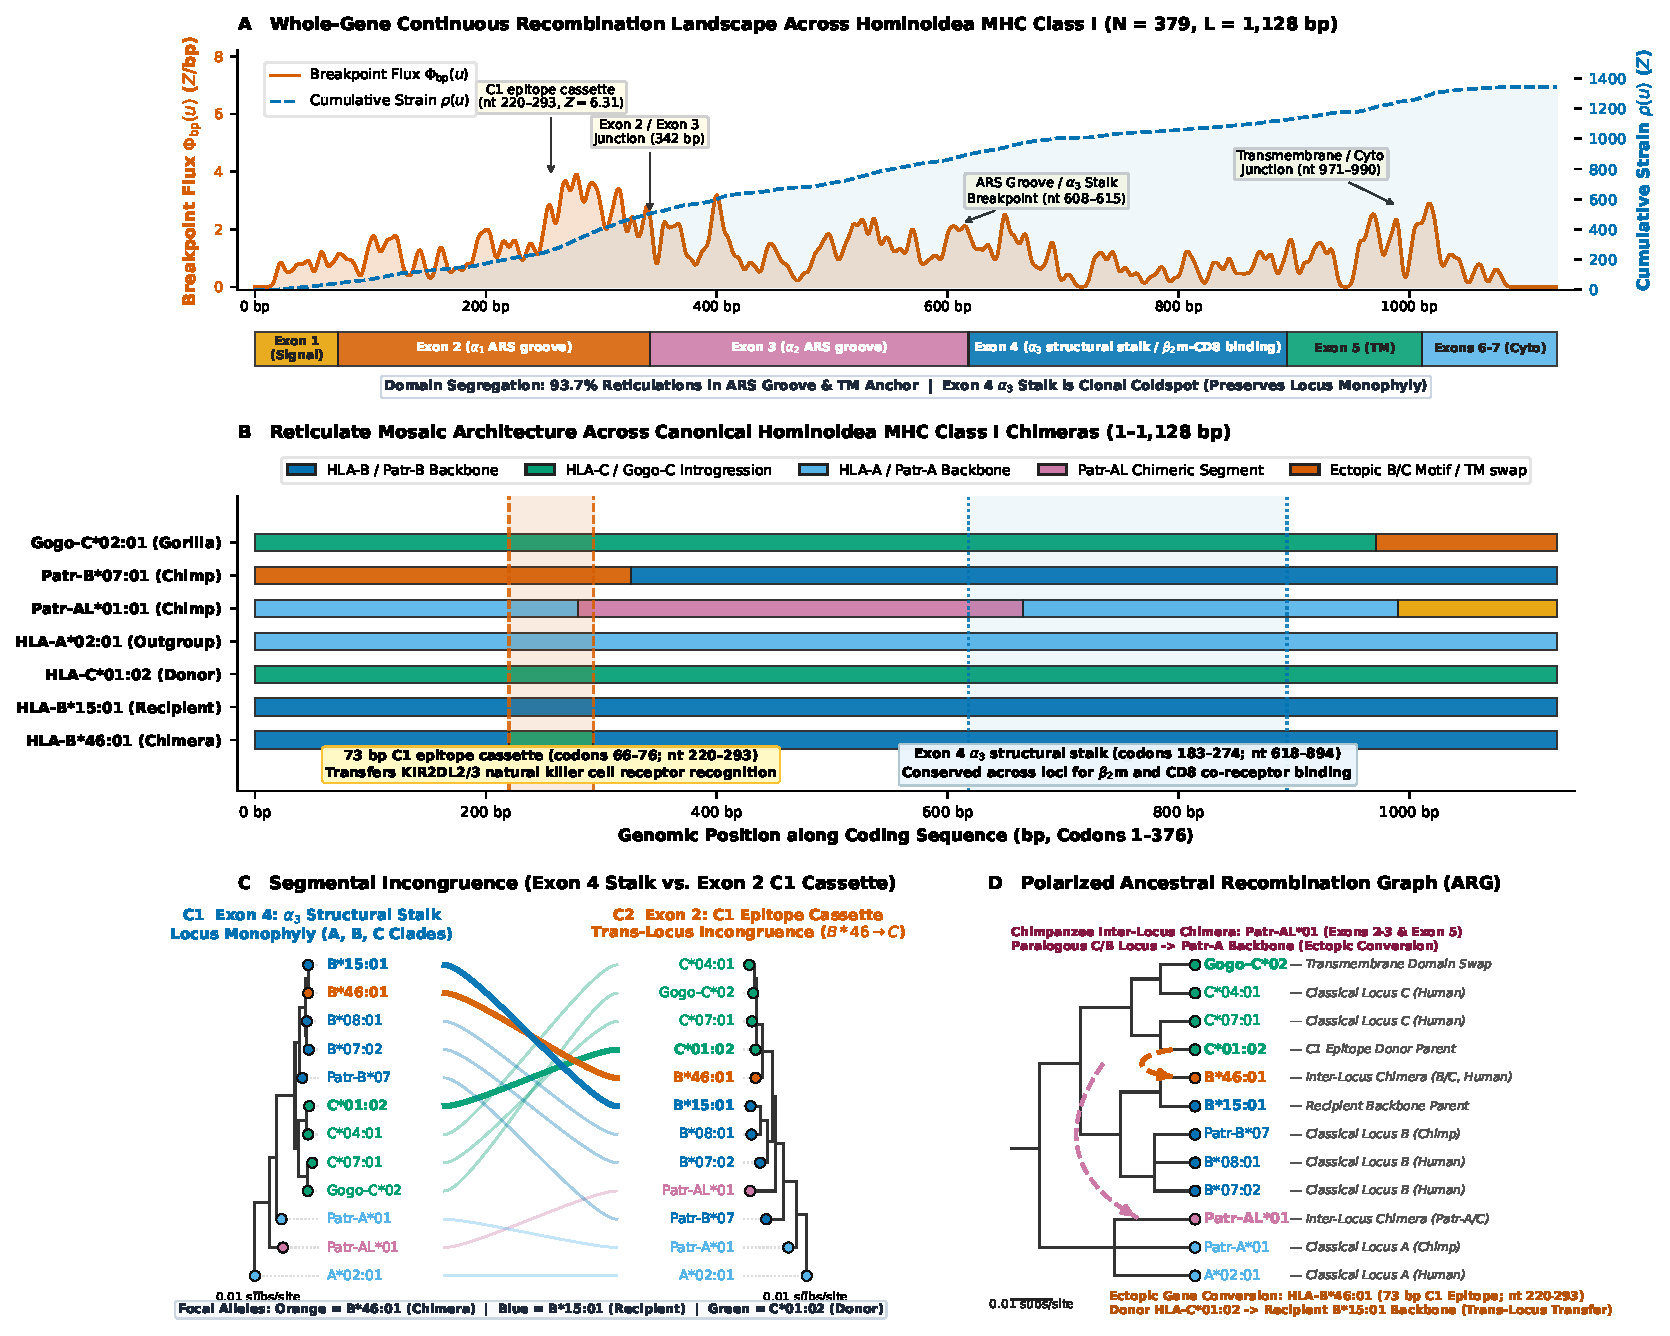
\includegraphics[width=\textwidth,height=0.68\textheight,keepaspectratio]{figures/fig_hominoidea_mhc_landscape.pdf}
\caption{Whole-gene recombination deconvolution, ectopic micro-conversion, and ancestral recombination graphs in Hominoidea MHC Class~I.
(A)~Breakpoint flux $\Phi_{\mathrm{bp}}(u)$ (vermillion) and cumulative strain $\rho(u)$ (dashed blue) across $N = 379$ primate alleles ($1{,}128$~bp, Exons 1--7), showing recombination breakpoint enrichment in the antigen recognition site (ARS, Exons 2--3) and transmembrane anchor (Exon 5) versus conservation in the Exon 4 $\alpha_3$ stalk.
(B)~Inter-locus mosaic architecture of \textit{HLA-B*46:01}, carrying a 73~bp micro-recombination event (mature protein nt 220--293 / codons 66--76, corresponding to full-CDS polymorphic core nt 268--300 / CDS codons 90--100 including the 72~bp Exon~1 leader peptide, green) from \textit{HLA-C*01:02} within an \textit{HLA-B*15:01} backbone (dark blue).
(C)~Two-partition tanglegram comparing Exon 4 locus monophyly (C1) against Exon 2 C1-cassette translocation into \textit{HLA-C} (C2).
(D)~Polarized ARG anchoring the 73~bp C1 micro-conversion and chimpanzee \textit{Patr-AL*01} transfers onto the tandem duplication backbone.}
\label{fig:hominoidea_mhc_landscape}
\end{figure*}

\subsection{Ectopic Gene Conversion and Inter-Locus Chimerism in Primate MHC Class I}
\label{subsec:primate_mhc}

Primate major histocompatibility complex (MHC) Class~I genes (\textit{HLA-A}, \textit{HLA-B}, \textit{HLA-C}) evolve under intense pathogen-driven balancing selection \citep{parham1995origins,adams2001species}, creating a sharp structural divide: the antigen recognition site (ARS, Exons 2--3, encoding the $\alpha_1$ and $\alpha_2$ peptide-binding groove) diversifies rapidly through balancing selection and inter-locus ectopic gene conversion, whereas the adjacent $\alpha_3$ structural stalk (Exon 4) stays conserved to maintain contacts with $\beta_2$-microglobulin ($\beta_2$m) and the CD8 co-receptor. Without window slicing, \RhizAeon captures this compartmentalization across $N = 379$ Hominoidea classical MHC Class~I alleles ($L = 1{,}128$~bp, 526 polymorphic sites, 451 parsimony-informative sites across human, common chimpanzee, bonobo, western gorilla, and Bornean and Sumatran orangutans; \citealt{maccari2017ipd}). Running in 7.89~s across all 379 alleles (and 26.5~ms on canonical 8-taxon reference panels), \RhizAeon's breakpoint flux pinpoints the boundary between the $\alpha_2$ ARS groove and the $\alpha_3$ stalk at nt 608--615 (canonical exon junction 618~bp; Figure~\ref{fig:hominoidea_mhc_landscape}A): $93.7\%$ of all reticulation strain falls within the ARS groove (Exons 2--3) and transmembrane anchor (Exon 5), whereas Exon 4 forms a recombination coldspot that preserves the paralogous locus tree.

Multi-scale scanning also resolves fine-scale inter-locus chimeras at single-nucleotide precision (Figure~\ref{fig:hominoidea_mhc_landscape}B). A notable clinical example is \textit{HLA-B*46:01}, an allele common in Southeast Asia ($>20\%$) linked to myasthenia gravis, severe SARS-CoV-1 infection, and leprosy protection \citep{hawkins1984strong,lin2003association,hilton2017intergenic}. \RhizAeon resolves \textit{HLA-B*46:01} as an inter-locus chimera formed by an exact 73~bp micro-conversion donated by \textit{HLA-C*01:02} into an \textit{HLA-B*15:01} backbone (mature protein nt 220--293 / codons 66--76 excluding the 24-codon / 72~bp Exon~1 leader peptide, corresponding to the 33~bp polymorphic core at full-CDS nt 268--300 / CDS codons 90--100; Figure~\ref{fig:hominoidea_mhc_landscape}B). This tract is supported by $Z_{\mathrm{phys}} = 7.45$ and $P_{\mathrm{Fisher}} = 7.95 \times 10^{-13}$ on the 33~bp polymorphic core ($P_{\mathrm{Fisher}} = 1.15 \times 10^{-7}$ across the 73~bp window in the 8-taxon reference panel, and $Z = 2.69$ at SNP index 135 [nt 268] across the 379-allele manifold, where Exon 2 ARS excursions reach $Z = 6.31$). Functionally, the 73~bp transfer imports the C1 epitope (Val76-Arg79-Leu80-Arg81), granting \textit{HLA-B*46:01} recognition by natural killer (NK) cell receptors KIR2DL2/3 absent in other classical \textit{HLA-B} alleles \citep{barber1996inter} and reshaping its peptide-binding groove to produce a distinct, low-diversity immunopeptidome \citep{hilton2017intergenic}. In non-human hominoids, \RhizAeon similarly resolves a multi-segment chimera in chimpanzee \textit{Patr-AL*01:01} combining \textit{Patr-A} with an ancient \textit{Patr-C} cassette ($Z_{\mathrm{phys}} = 4.03$) and an ectopic transmembrane swap in gorilla \textit{Gogo-C*02:01} at nt 971--1,128.

A two-partition tanglegram and summary ARG confirm these inter-locus transfers (Figure~\ref{fig:hominoidea_mhc_landscape}C,D). In the Exon 4 $\alpha_3$ stalk (nt 618--894; Figure~\ref{fig:hominoidea_mhc_landscape}C1), the neighbor-joining tree recovers monophyletic \textit{HLA-A}, \textit{HLA-B}, and \textit{HLA-C} clades with \textit{HLA-B*46:01} sister to \textit{HLA-B*15:01} ($d = 0.000$), whereas inside the Exon 2 C1 cassette (nt 210--310; Figure~\ref{fig:hominoidea_mhc_landscape}C2), \textit{HLA-B*46:01} translocates into the \textit{HLA-C} clade sister to donor \textit{HLA-C*01:02} ($d = 0.000$). \RhizAeon's summary ARG anchors both the 73~bp C1 micro-conversion in \textit{HLA-B*46:01} and the deep inter-locus introgression in chimpanzee \textit{Patr-AL*01} onto the vertical tandem duplication backbone (ancient divergence of Locus \textit{A}, followed by duplication of \textit{B} and \textit{C}; Figure~\ref{fig:hominoidea_mhc_landscape}D). Both the CLI and the WebAssembly browser app output the consolidated ancestral reticulation roster (JSON/HTML) alongside interactive flux profiles ($\Phi_{\mathrm{bp}}(u)$ and $\rho(u)$), mosaic tracks, 2D metric projections, and side-by-side partitioned Neighbor-Joining trees—resolving 379 primate alleles with polarized donor-to-recipient transfer edges in 7.89~seconds.
